We now describe the experimental setup used to evaluate the performance of CRQA and other methods for near real-time question answering.

\subsection{Experimental Setup: TREC LiveQA}
The experimental evaluation of our CRQA system was done on the official run of TREC LiveQA shared task, which happened on May 31, 2016.
All participating systems were running for 24 hours and received questions sampled from the live (real time) stream of questions, posted by real users to Yahoo! Answers platform.
In total, each system received 1,088 questions, and system responses were recorded by the organizers.

\begin{table}[ht]
\centering
\begin{tabular}{| p{7cm} | c | }
\hline
Name & Value \\
\hline
Number of questions received & 1088 \\
Number of completed assignments (15 mins each) & 889 \\
Average number of questions per assignment & 11.44 \\
Total cost per question & \$0.81 \\
Average number of answers provided by workers & 1.25 \\
Average number of ratings per answer & 6.25 \\
\hline
\end{tabular}
\caption{Aggregate statistics of crowdsourcing tasks}
\label{table:task_stats}
\end{table}

Overall statistics are provided in Table \ref{table:task_stats}.
As we can see, on average workers were able to provide at least one answer for each question, and each of the provided answers got 6 ratings.
Since the interface could show only 3 answers at a time, answers had different chances of being rated.
To investigate the effect of the order of the candidates posted for ratings on the quality of the final answer, in CRQA for each worker and each question we randomly selected one of the strategies: ordering answer candidates by their model rank or random shuffling of the candidates.
The system variant with shuffled candidates for rating was expected to obtain more diverse and comprehensive set of ratings, as we will investigate in the Analysis section.

\subsection{Answer Quality Evaluation}
\label{sec:experiments:answer-quality-evaluation}

The official results of the shared task will be available in November 2016 during the TREC conference\footnote{http://trec.nist.gov/}.
Meanwhile, we used traditional (batch-mode) crowdsourcing to obtain the quality labels for all answer candidates that were given to the workers during the task, as well as the answers provided by the workers.
In addition, on June 2, two days after the TREC LiveQA challenge has completed, we crawled the current answers provided by the community for the questions, used for the task.
All the answers for each question were randomly shuffled and rated on a scale from 1 (bad) to 4 (excellent) by workers hired on Amazon Mechanical Turk.
Existing research demonstrated, that such crowdsourced labels correlates well with the official ratings, provided by the professional NIST assessors \cite{savenkov_crowdsourcing2016a}.
Each answer was labelled by 3 different workers, and we averaged the scores to get the final quality labels for the candidates.


\subsubsection{Methods compared.}
We compared CRQA system against several baselines:
\begin{itemize}
\item \textit{Automated QA}: automated QA system described in Section~\ref{sec:system:auto}.
\item \textit{CRQA}: Automated QA system with Crowdsourcing, described in Section~\ref{sec:system:crowd}
\item \textit{Re-ranking by score}: a simplified version of CRQA re-ranking model, which select the answer with the highest average ratings, provided by the crowd workers.
\item \textit{Yahoo Answers}: traditional, non-real-time community question answering site (Yahoo Answers), from which the challenge question originated. The answers were collected two days after the challenge, thus allowing the Yahoo Answers community extra two days to collect the answers through traditional (community-based) crowdsourcing.
\end{itemize}

\subsubsection{Metrics.}
To evaluate the methods we used the metrics proposed by the organizers of the LiveQA task:
\begin{itemize}
\item \textbf{avg-score}: average score over all questions
\item \textbf{avg-prec}: average score over all answered questions
\item \textbf{succ@i+}: the fraction of answers with score i or greater (i=2..4)
\item \textbf{p@i+}: the number of answers with score i or greater (i=2..4) divided by the number of answered questions\footnote{Since for each answer we averaged 3 ratings by different workers, the number of answers with the average score of 4 is low}
\end{itemize}

\begin{table*}[ht]
\centering
\begin{tabular}{| p{3.7cm} | c | c | c | c | c | c | c | c |}
\hline
Method & avg-score & avg-prec & succ@2+ & succ@3+ & succ@4+ & prec@2+ & prec@3+ & prec@4+ \\
\hline
Automated QA & 2.321 & 2.357 & 0.697 & 0.297 & 0.026 & 0.708 & 0.302 & 0.026 \\
Re-ranking by score & 2.416 & 2.421 & 0.745 & 0.319 & 0.031 & 0.747 & 0.320 & 0.031 \\
Yahoo! Answers & 2.229 & 2.503 & 0.656 & 0.375 & \textbf{0.045} & 0.737 & \textbf{0.421} & \textbf{0.050} \\
CRQA (ratings + answers) & \textbf{2.550} & \textbf{2.556} & \textbf{0.799} & \textbf{0.402} & 0.034 & \textbf{0.800} & 0.402 & 0.034 \\
\hspace{5mm}worker ratings only & 2.432 & 2.470 & 0.750 & 0.348 & 0.030 & 0.762 & 0.354 & 0.031 \\
\hspace{5mm}worker answers only & 2.459 & 2.463 & 0.759 & 0.354 & 0.029 & 0.760 & 0.355 & 0.029 \\
\hline
\end{tabular}
\caption{Evaluation of the baselines and system answers quality based on the ratings of answers obtained via crowdsourcing. The scores are averaged over 100 different 50:50 splits of 1088 questions into the training and test set. The differences between average score and precision of CRQA and the original ranking are significant at p-value $<$ 0.01}
\label{table:performance}
\end{table*}

Table~\ref{table:performance} summarizes the performance of the baselines and our system.
As we can see, the average score and precision of answers generated by CRQA system is higher than the baseline ranking and even community answers on the Yahoo! Answers platform.
However, Yahoo! Answers community answers have higher percentage of \textit{``4 (excellent)''} scores.
Figure \ref{fig:score_histogram} shows the distribution of scores for the original system ranking, our crowdsourcing system and Yahoo! Answers.
Two peaks on the distribution of scores from Yahoo! Answers community suggest, that there are essentially two kinds of responses: non-useful (\textit{e.g.} spam) or excellent that fully answers the question.
In addition, around 20\% of the questions didn't get any answer from the community.
Automatically generated answers, on the contrary, are rarely empty, but on average provide only marginally relevant information, which often doesn't answer the questions, and therefore rated \textit{``2 (fair)''}.
The introduction of the crowdsourcing module allowed CRQA to cover a couple of percent of the questions, for which the automated system wasn't able to generate any candidates, as well as select better candidates when it was possible using crowd ratings.

\begin{figure}[h]
	\centering
	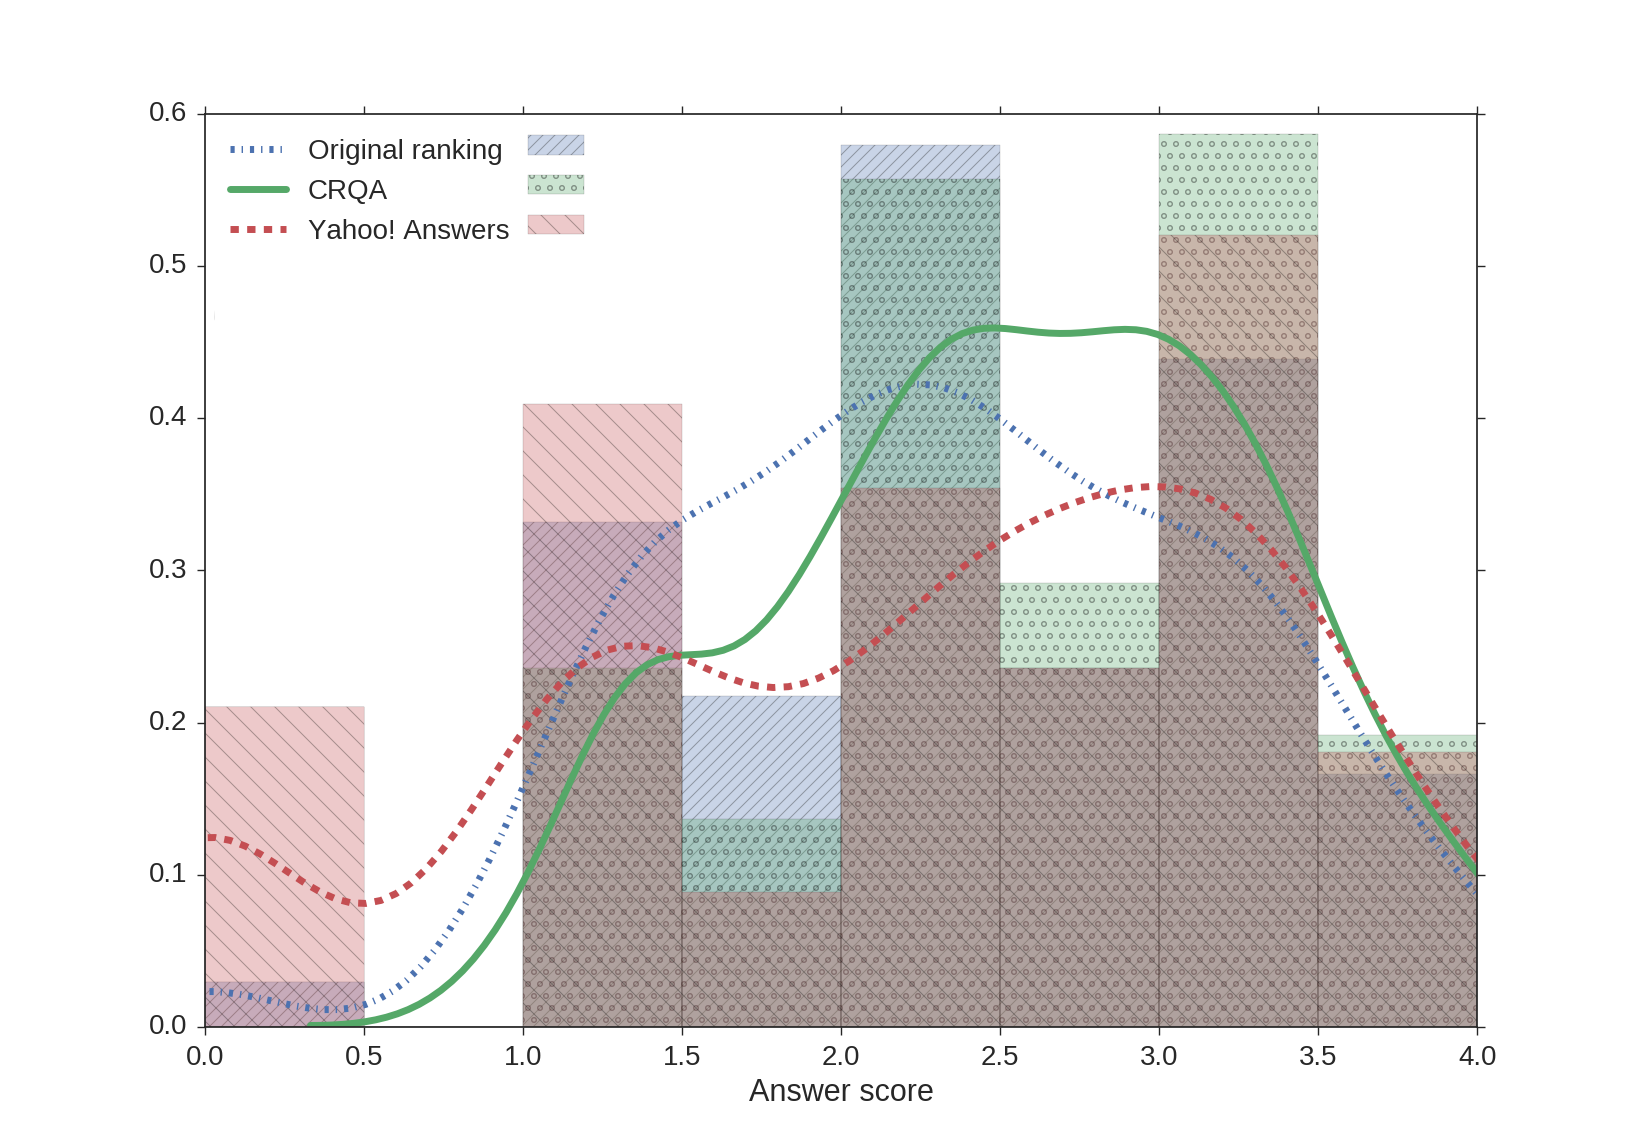
\includegraphics[width=0.5\textwidth]{img/score_hist}
	\caption{Histogram and kernel density estimation of answer scores for original candidate ranking, CRQA model re-ranking and Yahoo! Answers answers}
	\label{fig:score_histogram}
\end{figure}

Therefore, we can conclude, that crowdsourcing can effectively help automated QA system to improve the performance of question answering, by providing worker generated answers and rating existing candidates.

To summarize, our Crowd-powered Real-time Question Answering system substantially improves the quality compared to the baseline fully automated system, and generated answers are often even preferred to responses posted by CQA community.